\documentclass[conference]{IEEEtran}

\usepackage[dvips]{graphicx}
\usepackage{amsmath,amssymb}
\usepackage{algorithm}
\usepackage{algorithmic}
\usepackage{flushend}

\renewcommand{\sfdefault}{cmss}
\renewcommand{\rmdefault}{cmr}
\renewcommand{\ttdefault}{cmtt}

\usepackage{polyglossia}
\setdefaultlanguage[babelshorthands=true]{russian}

\usepackage{fontspec}
\setmainfont{FreeSerif}
\newfontfamily{\russianfonttt}[Scale=0.7]{DejaVuSansMono}

\usepackage{caption}
\usepackage{float}
\usepackage[colorlinks,filecolor=blue,citecolor=green,unicode,xetex]{hyperref}
\usepackage{cmap}
\usepackage{amsmath,amssymb}
\usepackage[mathcal]{euscript}
\hypersetup{colorlinks=true, linkcolor=blue, citecolor=blue, filecolor=blue, urlcolor=blue, pdftitle=1, pdfauthor=, pdfsubject=, pdfkeywords=}

\sloppy
\clubpenalty=0
\widowpenalty=0
\raggedbottom

\begin{document}
\title{TRIK Studio: Technical Introduction}
\date{}%date stay empty

\author{
	\IEEEauthorblockN{Dmitry Mordvinov}
	\IEEEauthorblockA{
		Department of Software Engineering \\
		St.-Petersburg State University \\
		St.Petersburg, Russia \\
		Email: mordvinov.dmitry@gmail.com
	}
\and
	\IEEEauthorblockN{Yurii Litvinov}
	\IEEEauthorblockA{
		Department of Software Engineering \\
		St.-Petersburg State University \\
		St.Petersburg, Russia \\
		Email: y.litvinov@spbu.ru 
	}
}

\maketitle

\begin{abstract}
This paper presents TRIK Studio --- an environment for visual (and textual) programming of robotic kits, which is used in educational organizations across Russia and Europe. First part of the article provides overview of the system --- its purpose, features, differences from similar programming environments, general difficulties of robot programming and solutions proposed by TRIK Studio. Second part presents implementation details of TRIK Studio and its most interesting components. This article combines five fields of study: robotics, domain-specific visual modelling, education, formal methods and methods of program analysis. Main contribution of this article is detailed technical description of TRIK Studio as a complex and successful open-source cross-platform robot programming environment written in C++/Qt, and first part of the article can also be interesting for teachers as it provides an overview of existing robot programming tools and related problems.
\end{abstract}

\section{Introduction}
Current state of school education in computer science turned out to be quite like Seymour Papert predicted it to be. In 1967 he introduced a virtual Logo turtle, that is used to teach students programming at schools even nowdays. It is less known that Papert in his experiments also used a mechanical robot turtle, that was controlled from a computer ~\cite{papert1980mindstorms}, and it made educational process much more entertaining. Today Papert's ideas are widely spread, a lot of schools are using robots to teach programming (for instance, in Russia robotics is a part of compulsory education program within the Technology course \cite{черёмухин2014внедрение,лучин2016внедрение}). Several robotics educational kits are used, including Lego Mindstorms NXT, Lego Mindstorms EV3 \footnote{LEGO Mindstorms homepage, URL: http://www.lego.com/en-us/mindstorms (accessed: 07.02.2017)}, 
TRIK\footnote{TRIK robotics platform homepage, URL: http://www.trikset.com/ (accessed: 07.02.2017)} etc.

Задача программирования робота, собранного из конструктора, сложнее, чем виртуальной <<черепашки>>: программы должны быть написаны в терминах мощностей моторов и значений с датчиков вместо конкретных перемещений и поворотов. Поэтому при внедрении таких конструкторов в учебный процесс большое внимание уделяется средствам их программирования. При этом довольно популярными являются визуальные языки, поскольку они нагляднее текстовых и проще в изучении. Программирование в таких средах осуществляется, в основном, <<перетаскиванием>> графических примитивов с помощью компьютерной мыши, иногда это дает возможность программировать роботов даже детям, которые еще не умеют читать. 

Популярность визуальных языков в образовательной робототехнике подчеркивается количеством сред программирования учебных роботов на таких языках. К самым известным отнесем Robolab~\cite{erwin2000lego}, NXT-G~\cite{kelly2010lego} и EV3-G~\cite{valk2014lego}, Scratch~\cite{resnick2009scratch} и Scratch-подобные среды (S4A~\cite{s4a}, mBlock~\cite{mblock}, Enchanting~\cite{enchanting}, ScrathDuino~\cite{scratchduino}, Blockly~\cite{blockly} и App Inventor~\cite{wolber2011app}, 12Blocks~\cite{12blocks}, Open Roberta~\cite{jost2014graphical}, Ardublock~\cite{ardublock}), среды программирования менее популярных конструкторов и роботов, такие, как Robo PRO~\cite{chang2006incorporating} для конструктора fischertechnik или Scribbler Program Maker для роботов Scribbler, а также среды программирования для дошкольников и учеников начальных школ Lego WeDo Software~\cite{mayerova2012pilot}, Create~\cite{cross2013visual}, Wonder~\cite{wonder}. В наши дни научная область образовательной робототехники представляет большой интерес в мире, о чем говорит, например, тот факт, что в 2010-х годах практически каждый ведущий университет мира занялся разработкой собственных решений. К примеру, в апреле 2016 года Гарвардский Университет представил платформу Root~\cite{root}, Университет Карнеги--Меллон занимается разработкой и продвижением проекта Arts\&Bots~\cite{cross2013visual}, Массачусетский технологический институт внес свой вклад созданием системы Scratch~\cite{resnick2009scratch}, и данный список на этом не иссякает. Подробный русскоязычный обзор всех вышеупомянутых сред можно найти в работе~\cite{mordvinov2016NONPUBLISHED}, в которой делается вывод о том, что несмотря на разнообразие всех инструментов в данной области, ни один из них не может удовлетворить требованиям многих образовательных учреждений. Подавляющее большинство таких сред реализуют только наиболее общую и необходимую функциональность (редактор визуальных диаграмм и возможность исполнить их на роботе с отладкой на компьютере или в автономном режиме), однако в них отсутствуют более специализированные средства обучения программированию, например, возможность генерации читаемого кода по визуальной диаграмме для облегчения <<перехода>> с визуальных языков на текстовые, возможность отладки программы на виртуальном симуляторе робота или встроенные средства проверки корректности выполнения задания, что автоматизировало бы часть обязанностей преподавателя. В случае, если такие возможности присутствуют в системе, то не все сразу, и все такие среды проприетарны и не бесплатны: их пользователи могут попасть в ситуацию <<vendor lock-in>>, не говоря уже о том, что многие учебные заведения не могут позволить себе покупку дорогостоящих лицензий. 

Практически все вышеупомянутые языки реализуют модель вычисления с передачей управления (\textit{control flow}). Такая модель легче воспринимается людьми, поэтому ее разумнее использовать в образовательных целях. Тем не менее, модель потока управления не самая удачная для программирования роботов. Дело в том, что роботы по своей природе реактивны: программа управления роботом представляет собой преобразование сигналов с датчиков в импульсы на приводы. Реактивные модели хорошо описываются так называемыми \textit{языками программирования потоков данных} (\textit{dataflow languages})~\cite{johnston2004advances}, в которых программа представляется множеством <<черных ящиков>>, соединенных каналами данных. Каждый такой <<ящик>> (далее, \textit{блок}) имеет фиксированный набор входов и выходов, его работа состоит в преобразовании данных на входе в данные на выходе (далее данные, посылаемые по каналу, будем называть \textit{токенами}). К примеру, каждый датчик робота в такой схеме описывается всего одним блоком, который отправляет в выходные каналы токены значений с датчика. При этом многие исследователи отмечают удобство визуальных потоковых языков по сравнению с текстовыми~\cite{johnston2004advances}, в частности, из-за наглядной визуализации самих потоков данных.

Идея использования потоковых языков программирования в робототехнике не нова, она реализована практически в каждом инструменте для визуального программирования промышленных и лабораторных систем автоматизации. К таким системам отнесем LabVIEW от компании National Instruments~\cite{kodosky1991visual}, систему Simulink~\cite{dabney2004mastering}, а также среду визуального программирования роботов Microsoft Robotics Developer Studio~\cite{jackson2007microsoft}. Все упомянутые системы хорошо решают задачу автоматизации, имеют мощные инструментарии (например, Microsoft Robotics Developer Studio используется на серверах в широко известной социальной сети MySpace~\cite{scherotter2009ccr}), однако весьма сложны в изучении и даже громоздки, поэтому если и применяются в образовании, то гораздо чаще в университетском~\cite{stefanovic2011labview,yi2005labview}. К примеру, школьные образовательные эксперименты с LabVIEW были популярны в конце 1990-х годов~\cite{cyr1997low,portsmore1999robolab}, что привело к появлению образовательных адаптаций среды (таких, как Robolab), в которых, в частности, модели потоков данных была предпочтена модель потока управления. Таким образом, в контексте образования появляется другая проблема --- <<разрыв>> между упрощенными учебными языками и более элегантными, но сложными потоковыми. Исследователи пытаются адаптировать потоковую модель для образовательной робототехники,     к примеру, новозеландской исследовательской группой был предложен язык RuRu~\cite{diprose2011ruru}. Тем не менее, готовых сред программирования на визуальном потоковом языке, применяемых в образовании, все еще не существует.

Данная работа описывает новый инструмент программирования роботов TRIK Studio, являющийся попыткой решения вышеописанных проблем. Успешность их решения косвенно подтверждается практическими применениями: на данный момент TRIK Studio широко применяется в российском образовании (десятки школ и тематических кружков), известны применения в образовательном процессе европейских стран (Англии и Франции), отдельные пользователи есть на каждом обитаемом континенте мира. Описание будет дано с технической стороны, образовательные аспекты в данной статье затронуты в гораздо меньшем объеме.

\section{General description}
\label{chapter:generalDescription}

TRIK Studio --- среда визуального и текстового программирования образовательных конструкторов роботов. TRIK Studio появилась как развитие проекта кафедры системного программирования СПбГУ QReal:Robots~\cite{terekhov2013sreda}. В официальной версии имеется поддержка конструкторов Lego Mindstorms NXT, Lego Mindstorms EV3 и ТРИК. Каждый из этих конструкторов может быть запрограммирован на одном из двух визуальных языков --- более простом, построенном на модели потока управления, или более сложном языке программирования потоков данных --- либо на одном из нескольких текстовых. Для Lego NXT доступны языки NXT OSEK C и русскоязычная версия C (для облегчения изучения текстовых языков), для ТРИК --- JavaScript, F\#~\cite{kirsanov2014robotics} или PascalABC.NET~\cite{doliner2014basics}, для Lego EV3 поддержан единственный официальный язык программирования стандартной прошивки --- байткод виртуальной машины EV3.

Программа на визуальном языке (\textit{визуальная диаграмма}) может быть исполнена в трех режимах: 
\begin{itemize}
    \item отладка на симуляторе,
    \item отладка на компьютере с посылкой пакетов на робота по одному из физических каналов (USB, Bluetooth, Wi-Fi, см. главу~\ref{chapter:communications}),
    \item режим генерации кода на текстовом языке (одном из вышеупомянутых) с последующим автономным исполнением его на роботе. 
\end{itemize}

В режиме отладки на симуляторе диаграмма интерпретируется на двумерной имитационной модели робота (см. раздел~\ref{chapter:2dModel}). Пользователь имеет возможность нарисовать двумерную модель мира из стенок, цветных элементов и разметки регионов. Такая возможность, по отзывам пользователей, является очень удобной для первоначальной отладки программы перед каким-либо взаимодействием с роботом. Опыт использования показал, что в редакторе модели мира можно создать большинство полей и полос препятствий, используемых на соревнованиях по спортивной робототехнике. Наличие симулятора дает возможность обучения программированию и кибернетике в образовательных учреждениях, которые не имеют реальных роботов. Существует также экспериментальная поддержка отладки на трехмерном симуляторе роботов V-Rep~\cite{rohmer2013v}.

Отладка на компьютере с посылкой команд роботу (режим \textit{интерпретации} в терминах среды) удобна для отслеживания поведения программы на целевом устройстве в реальном времени. В режиме интерпретации можно отслеживать значения переменных в соответствующем окне среды (аналогичному, например, окну поддержки отладчика gdb в различных текстовых IDE), а также строить в реальном времени графики значений с датчиков.

Режим генерации кода позволяет перейти от визуального представления программы к текстовому. Тестовый код отображается во встроенном редакторе qscintilla\footnote{https://riverbankcomputing.com/software/qscintilla/intro (дата обращения: 14.05.2016)}, который обладает возможностью полноценного редактора кода (подсветка синтаксиса, автодополнение, подсветка скобок, отмена/повтор и т.д.). В дистрибутив среды входят все необходимые инструменты для построения и передачи программ на робота (набор кросскомпиляторов, WinSCP, Putty и т.д.), поэтому процесс компиляции и взаимодействия с контроллерами роботов остается полностью <<прозрачным>> для пользователей (пользователи-новички до определенного момента даже не догадываются о его существовании).

Пользовательский интерфейс среды представлен на рисунке~\ref{image:TS_interface}. На нем запечатлен момент отладки программы выезда робота из лабиринта на двумерном симуляторе.

\begin{figure*}[ht]
    \centering
    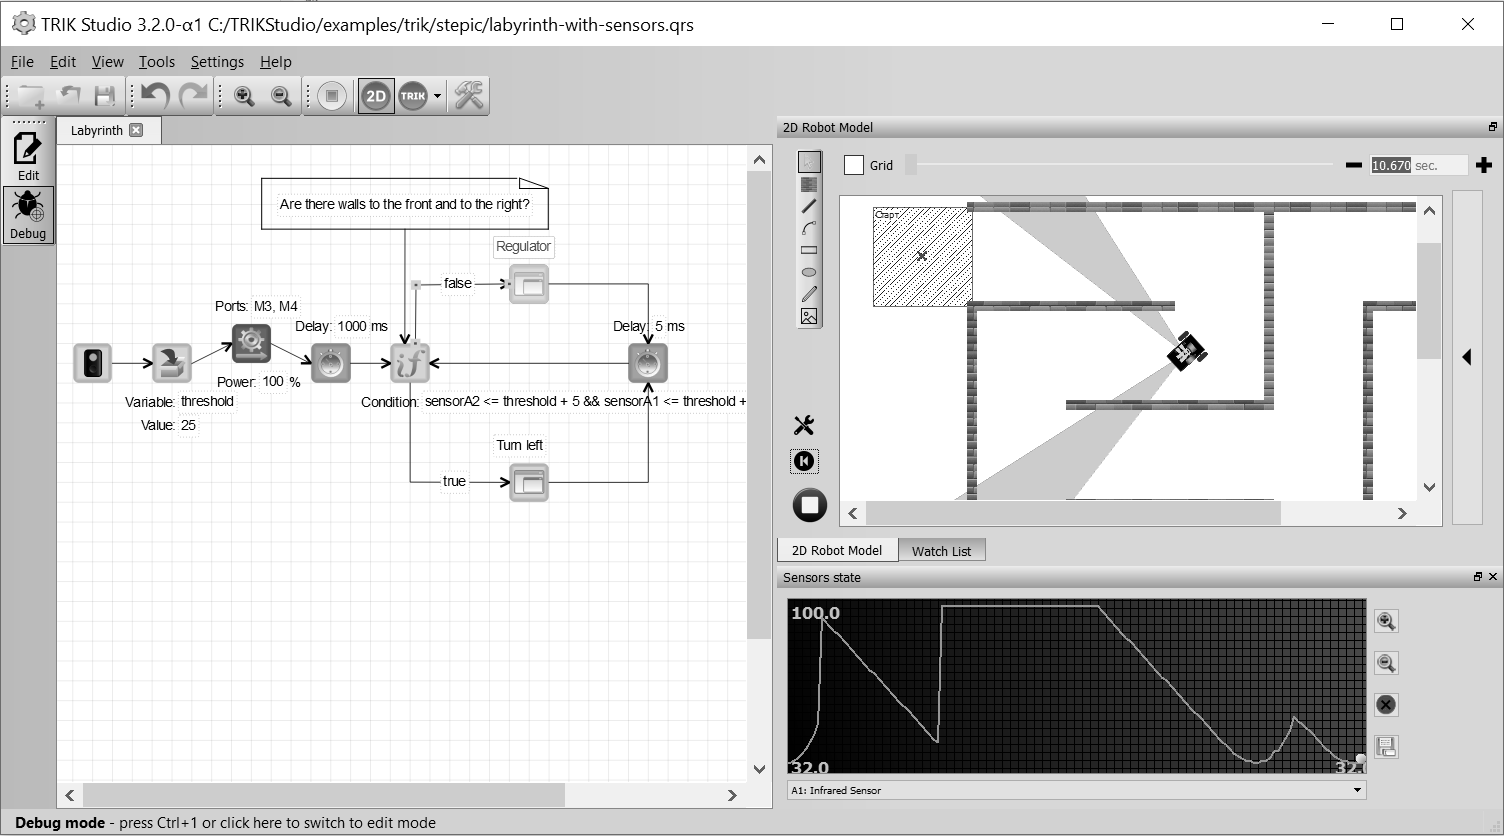
\includegraphics[width=\textwidth]{TS_CF_Labyrinth.png}
    \caption{Интерфейс TRIK Studio}
    \label{image:TS_interface}
\end{figure*}

В режиме двумерной симуляции доступна возможность автоматической проверки задач (см. раздел~\ref{chapter:constraintsChecker}). Программа проверки пишется на внутреннем событийном текстовом языке, файл с сохранением модели симулируемого мира и программы проверки затем может распространяться как задача для учеников. На основе этой системы был запущен курс дистанционного обучения на платформе Stepik\footnote{https://stepik.org/s/7qe3xj4Z  (дата обращения: 14.05.2016)} с видео-лекциями по основам кибернетики, робототехники и использованию среды TRIK Studio, множеством небольших тестов и 20 задачами образовательной робототехники. Каждая задача может быть скачана, решена и проверена в TRIK Studio на локальном компьютере и сдана на сервер, где система проверки запустит решение на своих тестах (подобно формату решения задач на соревнованиях ACM ICPC).

Среда написана на языке C++ с инструментарием Qt\footnote{https://www.qt.io/ru/ (дата обращения: 14.05.2016)}, поэтому является кроссплатформенной (доступны установочные пакеты под Windows, Linux и Mac OS X). При этом, даже несмотря на то, что официальные драйвера для Lego NXT не доступны для Linux и Mac OS X x64, в TRIK Studio существует собственная их реализация, подробнее см. главу~\ref{chapter:communications}. Среда полностью бесплатна, имеет открытый исходный код и распространяется под лицензией Apache License 2.0\footnote{http://www.apache.org/licenses/LICENSE-2.0 (дата обращения: 14.05.2016)}.

Описанные достоинства выгодно выделяют TRIK Studio на фоне всех аналогов. Фактически, среди упомянутых во введении систем, применяемых в школьном образовании, лишь среда 12Blocks обладает приближенной функциональностью, однако генерирует не читаемый код (для Lego NXT), не имеет средств проверки задач, является платной и не русифицирована. Основные недостатки TRIK Studio на данный момент --- это слабая методическая поддержка среды, ограничивающаяся лишь справкой на русском язык, набором примеров и упомянутым курсом дистанционного обучения. Существуют и другие, более мелкие отрицательные особенности, о которых будет упомянуто в соответствующих разделах ниже.

Остаток статьи будет построен следующим образом. В главах~\ref{chapter:controlFlowLanguage} и~\ref{chapter:dataFlowLanguage} будут кратко описаны визуальные языки TRIK Studio и их интерпретаторы. Глава~\ref{chapter:commonArchitecture} дает общее представление об архитектуре среды. Дальнейшие главы будут посвящены конкретным подсистемам TRIK Studio. Общие сведения о реализации механизмов коммуникации с роботами даны в главе~\ref{chapter:communications}. Описания интерпретаторов визуальных языков в системе даны в главе~\ref{chapter:interpreters}. Наиболее интересные детали реализации генераторов в текстовые языки из диаграмм потока управления представлены в главе~\ref{chapter:generators}. В разделе~\ref{chapter:parser} описывается подсистема синтаксического анализа текстовой части языка. В главе~\ref{chapter:2dModel} рассказывается об особенностях реализации подсистемы двумерного имитационного моделирования, далее, в главе~\ref{chapter:constraintsChecker} описан язык описания программ автоматической проверки заданий, исполняемых на этой подсистеме. Наконец, заключительная глава подводит итоги работы.

\section{Visual language for beginners}
\label{chapter:controlFlowLanguage}

Из всего множества языков, на которых в TRIK Studio можно программировать роботов, наиболее часто используется упрощенный визуальный язык, основанный на модели потока управления (рис.~\ref{image:TS_CF_Example}). Язык является графовым, т.е. программирование на нем ведется в терминах узлов (\textit{блоков}) и связей, соединяющих их в поток управления. Для создания программы пользователь перетаскивает необходимые ему блоки на сцену редактора, правит их свойства и соединяет стрелками. Каждый блок выполняет последовательность элементарных комманд и передает управления по исходящим от него стрелкам (возможно, не всем).

Блоки в описываемом языке можно поделить на четыре группы.
\begin{itemize}
    \item В первую группу включаются блоки поддержки основных алгоритмических конструкций, такие как блоки начала и конца исполнения программы или подпрограммы, ветвления, организации арифметического цикла, выбора (switch), распараллеливания и работы с параллельными задачами (их слияния и принудительного завершения), вызова подпрограммы и блок текстового программирования на встроенном языке.
    \item Вторая группа --- блоки работы с периферийными устройствами робота. Сюда включаются элементарные действия, не требующие ожидания. К примеру, это блоки подачи импульсов на моторы, проигрывания звука, блоки работы с видео-зрением робота, синтезирования речи по заданной строке, управления счетчиками оборотов и лампочками на панелях контроллеров роботов, посылки сообщения на другого робота (часть поддержки мультиагентного взаимодействия), работы с файловой системой робота и т.д.
    \item Следующая группа включает в себя блоки, <<замораживающие>> исполнение текущего потока. Сюда входит блок ожидания заданного количества миллисекунд (аналог функции \texttt{msleep}), блоки ожидания желаемого значения с какого-либо датчика или пульта операторского управления роботом и блок ожидания сообщения с другого робота.
    \item Наконец, в четвертую группу входят блоки рисования графических примитивов на дисплее робота. К таким графическим примитивам относятся прямые линии, прямоугольники, эллипсы, дуги, текст, картинки, возможно управление цветом и толщиной кисти рисования, цветом заливки фона. В эту группу включены также специальные блоки управления маркером для рисования в двумерном симуляторе траектории перемещения робота, что позволяет решать в среде класс задач, предлагаемых различными популярными двумерными исполнителями, такими, как <<Черепашка Logo>> или <<Чертежник>>.
\end{itemize}

\begin{figure*}[ht]
    \centering
    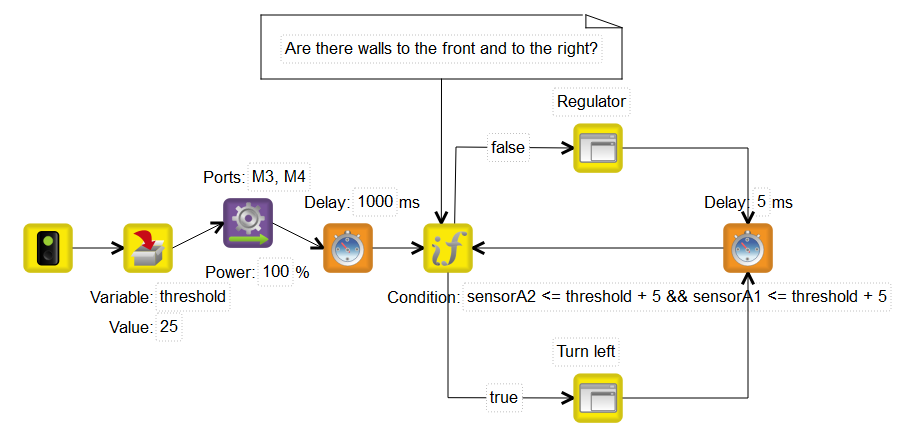
\includegraphics[width=0.8\textwidth]{TS_CF_Labyrinth_Diagram.png}
    \caption{Программа выхода из лабиринта по правилу правой руки. Первые четыре блока инициализируют программу: устанавливают константу порога близости стены, включают моторы робота, после чего робот продолжает движение одну секунду, чтобы заехать в лабиринт. Вторые четыре описывают главный цикл управления. Через каждые десять миллисекунд робот проверяет с помощью инфракрасных датчиков, может ли он продолжать движение вперед или направо (условие \texttt{sensorA2 <= threshold \&\& sensorA1 <= threshold}). Если движение возможно, то оно будет осуществляться посредством пропорционального регулирования значений правого датчика (подпрограмма <<Регулятор>>), если стены есть и слева, и справа, то робот поворачивается на 90 градусов влево (подпрограмма <<Налево>>)}.
    \label{image:TS_CF_Example}
\end{figure*}

Свойства каждого блока могут быть отредактированы как на самой сцене редактора, так и на отдельной панели редактора свойств. Во всех свойствах блоков, где это уместно, имеется возможность задать вычислимое значение на встроенном в TRIK Studio текстовом языке --- статически типизируемом диалекте языка Lua\footnote{http://www.lua.ru/ (дата обращения: 14.05.2016)}. Модуль синтаксического разбора этого языка написан с применением библиотеки парсер-комбинаторов для языка C++ стандарта 2011 года, созданной также в рамках проекта TRIK Studio. Вывод типов узлов результирующего абстрактного синтаксического дерева осуществляется алгоритмом Хиндли-Милнера~\cite{damas1982principal} с незначительными упрощениями.

Для реализации визуального языка был применен \textit{предметно-ориентированный подход} (\textit{DSM-approach})~\cite{koznov2008}. Редактор языка был создан при помощи DSM-платформы QReal~\cite{qrealMeta,kuzenkova2013qreal}. На визуальном метаредакторе DSM-платформы была описана метамодель языка, по ней которой средствами платформы был сгенерирован подключаемый модуль с редактором визуального языка. Результатом подключения такого модуля к ядру DSM-платформы является полноценная среда визуального программирования на языке, описанном метамоделью. Эта среда <<наследует>> все преимущества DSM-платформы, включая современный пользовательский интерфейс, поддержку рисования элементов жестами мышью~\cite{osechkina2010gestures,osechkina2012multistroke}, операции отмены-повтора в редакторе, возможности копирования-вставки групп элементов, изменения масштабов сцены редактора, различные способы рисования и отображения связей между элементами, панели-обозреватели моделей, поддержка особого режима работы на сенсорных-экранах и т.д. По отзывам пользователей, по эргономичности и современности визуальный редактор TRIK Studio превосходит многие аналоги, при этом время на создание первой версии визуального редактора заняло порядка трех человеко-дней. Все это говорит о разумности выбора DSM-платформы QReal в качестве базовой технологии, однако отметим, что во время написания инструментальной поддержки TRIK Studio в ядро DSM-платформы было внесено множество улучшений и исправлений.

\section{Visual language for advanced users}
\label{chapter:dataFlowLanguage}

Для пользователей, освоивших программирование на языке с передачей управления, в среде существует возможность программирования на более сложном, но более удобном визуальном языке. Этот язык построен на модели потока данных (\textit{dataflow model}). В отличие от предыдущего языка, где управление в программе явно передается по стрелкам, блоки в данном языке исполняются параллельно, обмениваясь друг с другом токенами по каналам данных. К примеру, у программы на потоковом языке может быть сразу несколько точек входа (чаще всего, это датчики робота, которые посылают данные далее по цепочке их обработки), в то время как у каждой программы на языке с передачей управления есть лишь одна входная точка. Аналогично предыдущему, потоковый язык содержит блоки поддержки основных алгоритмических конструкций, блоки взаимодействия со всеми устройствами роботов, блоки рисования и т.д. Как правило, диаграммы на потоковом языке получаются лаконичнее, чем аналогичные диаграммы на языке с передачей управления. К примеру, на рисунке~\ref{image:alongTheBox_CF_DF} пропорциональный регулятор для следования вдоль стены на языке с передачей управления сопоставлен пропорционально-дифференциальному регулятору на потоковом языке.

\begin{figure}[ht]
    \centering
    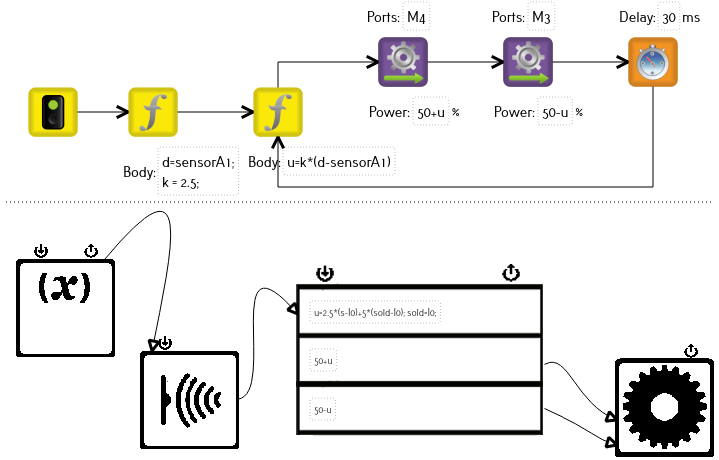
\includegraphics[width=\columnwidth]{TS_AlongTheBox_Comparison.png}
    \caption{Регуляторы на двух языках}
    \label{image:alongTheBox_CF_DF}
\end{figure}

Для упрощения изучения <<продвинутого>> языка в нем сохраняется концептуальная совместимость с моделью потока управления. Блоки здесь также могут быть выстроены в цепочку с явной передачей управления, для этого на большинстве блоков есть специальный порт активации, который игнорирует приходящие на него данные и попросту <<включает>> блок подобно тому, как это происходит в языке с передачей управления. Поначалу программирование на нем может вестись сходно с тем, как оно велось на языке для начинающих, и лишь с приходом должного опыта пользователь будет выражать свои идеи меньшим количеством блоков. 

Выразительная сила языка позволяет описывать на нем известные в робототехническом сообществе подходы к построению сложных систем управления роботов, такие как категориальная архитектура, предложенная Родни Бруксом~\cite{brooks1986robust}, архитектура <<колония>> Джонатана Коннелла~\cite{connell1989colony}, схема поведенческой навигации Рональда Аркина~\cite{arkin1987motor}, или распределенная схема навигации DAMN~\cite{rosenblatt1997damn}. Доказательство этих фактов является скорее материалом для отдельной статьи и здесь приведено не будет (при желании читатель может убедиться в этом на собственном опыте). Близкие идеи на эту тему могут быть найдены в статье английских исследователей~\cite{simpson2009toward} и диссертации~\cite{banyasad2000visual}.

Следует отметить, что на момент написания статьи поддержка потокового языка в среде реализована в экспериментальном режиме и не входит в официальную версию, распространяемую между конечными пользователями. Исходный код его редактора и инструментальной поддержки находится в открытом доступе\footnote{https://github.com/ZiminGrigory/qreal/tree/DFVPL (дата обращения: 14.05.2016)} и может быть собран вместе с исходным кодом TRIK Studio.

\section{General architecture}
\label{chapter:commonArchitecture}

Цель данной главы --- структурирование информации предыдущих разделов в виде архитектурного описания: большинство описываемых здесь деталей в каком-либо виде уже были упомянуты выше. Все диаграммы, представленные в данной главе абстрагированы от множества деталей, которые, хоть и представляют интерес в контексте данной статьи, здесь представлены не будут из соображений краткости.

На рисунке~\ref{image:commonTSArch} представлена часть общей архитектура среды TRIK Studio. Как из него видно, система разбита на несколько <<слоев>> абстракции. Каждый <<слой>> содержит код, реализующий сложные элементы функциональности среды и при этом имеет свой строго определенный и задокументированный API. На самом низком уровне такими <<слоями>> являются библиотеки взаимодействия с реальными и виртуальными роботами. На основе такого взаимодействия строится иерархия устройств робота (датчиков, приводов, дисплеев, динамиков, пультов управления, кнопок на контроллере и т.д.), из которых, в свою очередь, составляется описание модели того или иного конструктора роботов. Описания модели роботов группируются в подключаемые к ядру TRIK Studio модули, они используются другими подсистемами TRIK Studio (интерпретаторами и генераторами, которые также представляют собой подключаемые к ядру TRIK Studio модули).

Ядро TRIK Studio, в свою очередь, является подключаемым к DSM-платформе QReal модулем\footnote{Таким образом, в проекте реализована двухуровневая схема подключаемых модулей, подобно тому, как это сделано в системе ReSharper от компании JetBrains: ReSharper может расширяться подключаемыми модулями, при этом сам является подключаемым к Visual Studio модулем}. Оно подстраивает интерфейс QReal под себя, добавляя к нему множество панелей и окон, таких, как окно двумерного симулятора, панели конфигурирования датчиков робота, просмотра их значений и построения графиков и т.д.; подгружает все описания моделей роботов и отвечает за их рассылку всем необходимым подсистемам, предоставляет пользователю информацию о работе процесса генерации и интерпретации, и т.д. Наряду с ядром инструментальной поддержки TRIK Studio, к ядру QReal подключаются модули, описывающие редакторы визуальных языков, которые сгенерированы самой платформой QReal. Подробности про подсистемы более низкого уровня на рис.~\ref{image:commonTSArch} даны в главах ниже.

\begin{figure*}[ht]
    \centering
    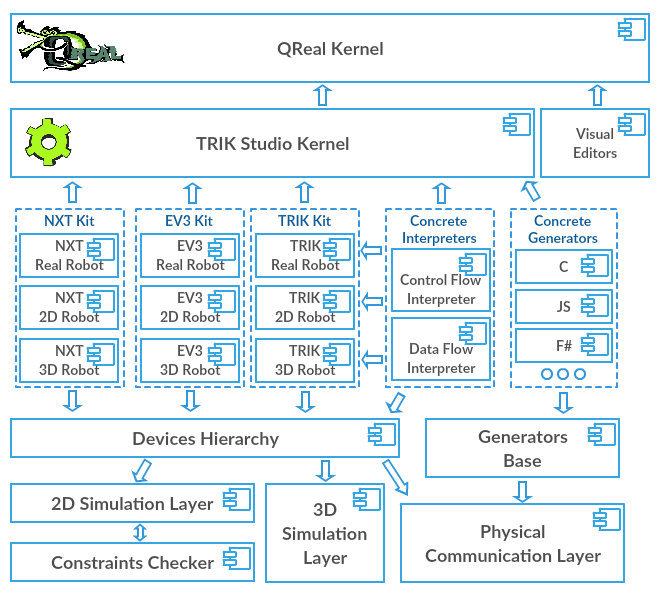
\includegraphics[width=0.6\textwidth]{TS_Common_Architecture.png}
    \caption{Общая архитектура системы}
    \label{image:commonTSArch}
\end{figure*}

Как можно заметить, вся среда построена на принципе подключаемых модулей. Отметим, что такая идея позволила сделать более гибкой систему конфигурирования установки: пользователь может выбрать, какие компоненты ему интересны, а остальные отключить (например, если у него есть только конструктор Lego EV3, то ему не нужны модули поддержки конструкторов Lego NXT и TRIK, в таком случае к нему на компьютер даже не попадут файлы, эту поддержку предоставляющие). Более того, такой подход хорошо совместим с пакетной организацией систем установки программ на различные дистрибутивы Linux. Это хорошо и с архитектурной точки зрения, так как исчезает большинство зависимостей между компонентами --- ядро TRIK Studio, к примеру, <<минималистично>>, оно <<не знает>> обо всех возможностях среды и содержит лишь общие для каждого робототехнического конструктора объекты и интерфейсы. API каждого <<слоя>> абстракции  зафиксировано и задокументировано, это может позволить создавать модули поддержки новых языков и конструкторов в среде даже независимым разработчикам из сообщества проекта.

\section{Communications with robot controllers}
\label{chapter:communications}

Одна из важных подсистем TRIK Studio --- это модуль взаимодействия с контроллерами роботов по тому или иному физическому протоколу. На рисунке~\ref{image:commonTSArch} это один из самых низких <<слоев>> абстракции среды. API модуля коммуникаций предоставляет следующие операции:

\begin{itemize}
    \item переключение текущего физического способа взаимодействия с целевым устройством (контроллером робота) между Bluetooth, USB и Wi-Fi,
    \item указание адреса устройства в терминах физического протокола (это может быть номер COM-порта в случае с взаимодействием по Bluetooth, IP-адрес или имя хоста в случае с взаимодействием по Wi-Fi),
    \item подключение-отключение к целевому устройству,
    \item посылка набора байтов на целевое устройство,
    \item события получения набора байтов с целевого устройства,
    \item события изменения статуса подключения (такие события вырабатываются, если связь с роботом установилась или разорвалась),
    \item события, оповещающие обо всех произошедших ошибках с локализованным их описанием.
\end{itemize}

Взаимодействие по USB происходит посредством библиотеки libusb\footnote{http://libusb.org/ (дата обращения: 14.05.2016)}, для реализации обмена по Bluetooth используется библиотека QextSerialPort\footnote{https://github.com/qextserialport/ (дата обращения: 14.05.2016)}, взаимодействие по Wi-Fi происходит поверх протоколов TCP и UDP посредством библиотеки QtNetwork, сложные протоколы коммуникации (такие как конфигурирование робота ТРИК перед запуском программы на исполнение) реализованы посредством Qt State Machine Framework. Процесс общения с целевым устройством происходит в отдельном потоке, чтобы не <<замораживать>> пользовательский интерфейс. Конкретные реализации механизмов коммуникации в подсистеме могут быть расширены и подменены другими компонентами <<извне>>, это используется, например, для совместимости TRIK Studio со стандартным драйвером Lego NXT. Отметим, что взаимодействие через него --- это не единственный способ общения с контроллером NXT по USB в TRIK Studio, в среде реализован собственный драйвер взаимодействия с Lego NXT, однако, в отличие от официального, работающий на всех поддерживаемых операционных системах через libusb.

\section{Interpreters}
\label{chapter:interpreters}

Интерпретатор преобразует визуальную диаграмму в последовательность команд на целевом устройстве (рис.~\ref{image:interpretersTSArch}). При этом иерархия устройств в системе построена таким образом, что не делается различий, реальное ли это устройство или симулируемое (рис.~\ref{image:devicesTSArch}). Каждое устройство представляет собой класс C++, содержащий код взаимодействия с целевым механизмом. Реализации устройств какого-либо конструктора находятся в соответствующих библиотеках подключаемых модулей. Для общения по физическим каналам устройства используют подсистему коммуникаций (гл.~\ref{chapter:communications}), для передачи команд двумерному и трехмерному симуляторам --- API этих симуляторов.

\begin{figure}[ht]
    \centering
    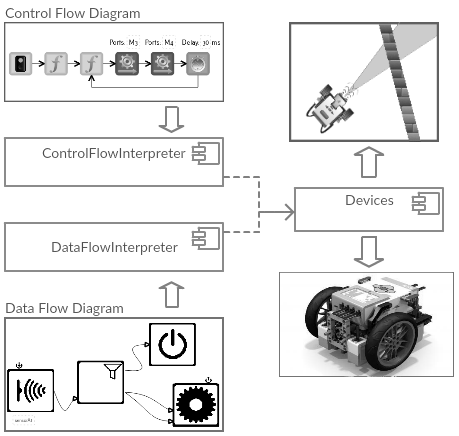
\includegraphics[width=0.9\columnwidth]{TS_Interpreter_Architecture.png}
    \caption{Общий принцип работы систем интерпретации}
    \label{image:interpretersTSArch}
\end{figure}

\begin{figure*}[ht]
    \centering
    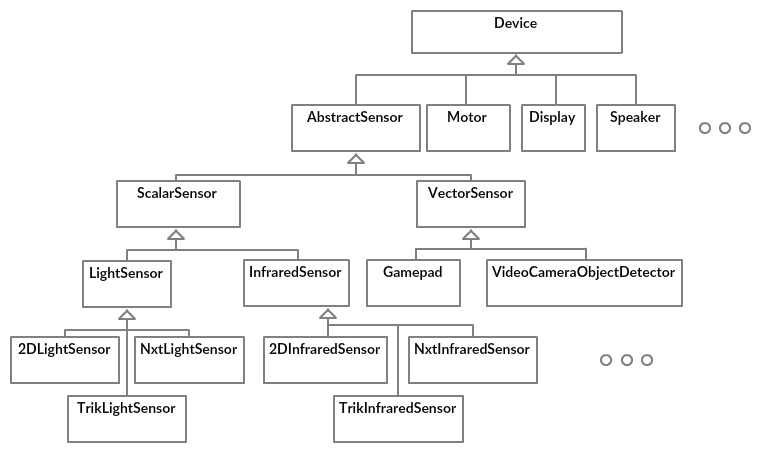
\includegraphics[width=0.7\textwidth]{TS_Devices_Architecture.png}
    \caption{Часть иерархии устройств в системе}
    \label{image:devicesTSArch}
\end{figure*}

Интерпретаторы, также как и вся система в целом, написан на языке C++ с использованием инструментария Qt. На вход подсистеме интерпретации поступает
описание созданной пользователем диаграммы в некотором внутреннем представлении. В среде реализовано два интерпретатора: интерпретатор языка для начинающих с передачей управления и интерпретатор потокового языка.

Интерпретатор первого языка находит на диаграмме начальный блок, и далее трассирует поток управления диаграммы в том порядке, как он задан стрелками. Текущий блок исполнения подсвечивается на визуальной диаграмме, чтобы пользователю был виден прогресс исполнения. Для каждого посещенного блока специальные фабрики интерпретатора создают объекты, которые реализуют его поведение. В общем случае, такой объект-реализация ищет среди готовых к работе устройств робота необходимые ему, вызывает соответствующие команды и передает управление следующим блокам по какой-либо исходящей ветке (которая определяется, опять-таки, самой реализацией блока). При этом не делается различий, является ли найденное устройство частью реального робота или симулируемым, таким образом, одна и та же подсистема интерпретации используется для исполнения диаграммы в двух режимах из трех (гл.~\ref{chapter:generalDescription}).

Если на каком-то шаге интерпретации повстречался блок распараллеливания, интерпретатор запускает новые потоки исполнения с соответствующих точек, создавая для каждого свой стек вызовов. Если встретился вызов подпрограммы, вычисляются ее параметры, укладываются на текущий стек вызовов, и далее процесс интерпретации повторяется рекурсивно. При достижении любого завершающего блока со стека снимается верхний фрейм, и исполнение продолжается с соответствующей точки на предыдущей диаграмме. Если при снятии очередного фрейма стек вызовов стал пустым, текущий поток исполнения считается завершенным. Таким образом, программа исполняется по мере того, как она <<открывается>> интерпретатору.

Отличительной чертой такой реализации является тот факт, что все изменения, вносимые пользователем на диаграмму во время процесса интерпретации, <<подхватываются на лету>>. Это является удобным, например, в случае подбора коэффициентов пропорциональности какого-либо регулятора, реализованного в программе. При этом процесс исполнения не изменившихся частей диаграммы оптимизирован: объекты-реализации блоков кэшируются в отдельную таблицу, то же происходит с абстрактными синтаксическими деревьями и информацией о выводе типов выражений на текстовом языке. Таким образом, если содержимое программы не меняется во время процесса интерпретации, повторная передача управления в ветки программы повлечет использование уже созданных сущностей. Валидация диаграммы также осуществляется <<на лету>>, в случае, если в диаграмме найдено некорректное место, пользователю отображается локализованное сообщение об ошибке. Последняя черта может рассматриваться как отрицательная, так как сообщение об ошибке появляется лишь в момент ее достижения в программе, что, впрочем, типично и для широко используемых текстовых интерпретируемых языков.

Интерпретатор потокового языка работает в два этапа. На первом, подготовительном этапе диаграмма проходит валидацию, создаются объекты-реализации элементарных блоков, преобразующие диаграмму в команды на устройствах роботов подобно тому, как это происходит в интерпретаторе языка, описанного в предыдущей главе. Объекты-реализации соединяются друг с другом посредством механизма сигналов и слотов инструментария Qt в соответствии с тем, как они соединены потоками данных на диаграмме; здесь оказался полезным паттерн проектирования <<издатель-подписчик>>. На втором этапе интерпретатор запускает на автономное исполнение каждый из блоков, в который не входит ни один поток данных, каждый из которых, в свою очередь, будет активировать блоки, соединенные с ним выходными потоками данных при выработке токенов. Исполнение блоков происходит псевдопараллельно с централизованной очередью сообщений (рис.~\ref{image:dsPseudoparallelism}). Это решение отличает данный язык от всех его промышленных аналогов (к примеру, в Microsoft Robotics Developer Studio диаграмма разворачивается в набор независимых веб-сервисов~\cite{jackson2007microsoft}), его причины состоят в узкой направленности языка на <<слабые>> контроллеры учебных роботов, в которых параллельное исполнение большого количества блоков затруднительно или вовсе невозможно. Тем не менее, в языке все же присутствует блок распараллеливания, который полезен, например, для выражения вышеупомянутых подходов к проектированию сложных систем управления. Такой блок может рассматриваться как механизм низкоуровневого управления вычислительными ресурсами в языке.

\begin{figure}[ht]
    \centering
    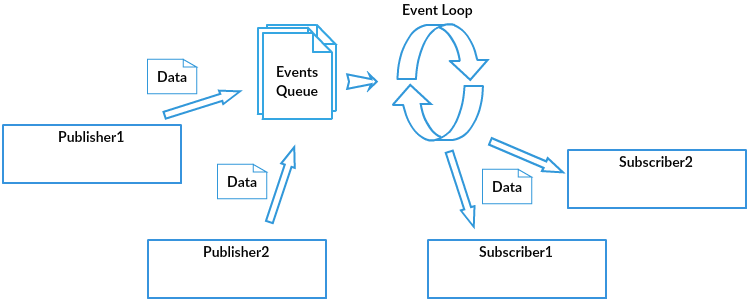
\includegraphics[width=\columnwidth]{DF_Interpretation_Process.png}
    \caption{Механизм исполнения потоковой программы в TRIK Studio}
    \label{image:dsPseudoparallelism}
\end{figure}

\section{Generators}
\label{chapter:generators}

Одна из наиболее важных и востребованных функций среды TRIK Studio --- генерация читаемого кода по визуальной диаграмме. По одной и той же диаграмме может быть сгенерирован код на любом поддерживаемом средой текстовом языке (C, JavaScript, F\#, Pascal, РуСи~\cite{тереховотечественные}, байткод ВМ EV3). Под визуальными диаграммами в данном разделе будем подразумевать программы на языке для начинающих (с передачей управления), под генераторами --- модули генерации кода по визуальным диаграммам именно этого языка.

Визуальная диаграмма состоит из блоков и стрелок, таким образом, описывает \textit{граф потока управления} программы~\cite{steven1997advanced}. Все основные алгоритмические конструкции (развилки, циклы, конструкции выбора и т.д.) складываются из стрелок. Например, чтобы задать бесконечный цикл, достаточно лишь провести стрелку от блока к одному из предыдущих, для описания циклов вида \texttt{while-do}, \texttt{do-while} или с инструкцией \texttt{break} внутри тела достаточно лишь провести одну из веток развилки из тела цикла к соответствующему блоку вне его. Очевидно, что одна стрелка на диаграмме соответствует инструкции \texttt{goto} в коде. Однако код, содержащий инструкции \texttt{goto} весьма труден для чтения человеком, тем более не подходит для обучения азам текстового программирования, поэтому следует избегать их появления в сгенерированном коде. Тем не менее, на TRIK Studio возможно написать программу, не выразимую общепринятыми алгоритмическими конструкциями, в таком случае появления инструкций \texttt{goto} в коде не избежать (существуют методы автоматического преобразования программы с goto в структурную программу, но результат их работы не лучше с точки зрения обучения текстовому программированию). С другой стороны, далеко не все современные текстовые языки поддерживают инструкцию \texttt{goto} (например, в языке JavaScript такой поддержки нет). Будем называть \textit{приводимыми} диаграммы, которые можно выразить стандартными алгоритмическими блоками (\texttt{if-then}, \texttt{if-then-else}, \texttt{while-do loop}, \texttt{do-while loop}, \texttt{while-break loop}, \texttt{switch}), код на текстовом языке, соответствующий структурированной диаграмме также будем называть \textit{структурированным}. В противном случае будем говорить, что диаграмма \textit{неприводима}, а код будем называть \textit{неструктурированным}. В случае, если диаграмму не удается сгенерировать в структурированный код, пользователю должно быть показано предупреждение.

Таким образом, реализация системы генераторов в TRIK Studio потребовала решения двух нетривиальных задач, которые сформулированы ниже в виде требований.

\begin{itemize}
    \item Система генераторов должна быть организована таким образом, чтобы добавление в систему генератора в новый текстовый язык занимало минимальное количество времени и усилий. По возможности, это должно быть по силам даже людям, не знакомым с кодом системы.
    \item Для каждого языка (где это возможно) система должна поддерживать два режима генерации: приводимые диаграммы должны быть сгенерированы в структурированный код, неприводимые --- в неструктурированный. При этом успешность структурирования диаграммы не должна зависеть от ее размера и сложности.
\end{itemize}

Первая задача является чисто архитектурной. Ее решение представлено на рисунке~\ref{image:generatorsArchitecture}. Основная идея --- разделение процесса генерации на два этапа. На первом диаграмма преобразуется в представление, независимое от целевого языка генерации --- \textit{семантическое дерево}. Семантическое дерево упорядочивает структуру графа потока управления до <<древесной>>, в независимости от того, является ли диаграмма приводимой или нет. В случае, если диаграмма приводима, родительский узел семантического дерева всегда соответствует блоку вычислений в целевом коде, дети --- инструкциям этого блока, среди которых нет \texttt{goto}. Опишем последовательность действий, отображенных на рисунке~\ref{image:generatorsArchitecture}.

\begin{figure*}[ht]
    \centering
    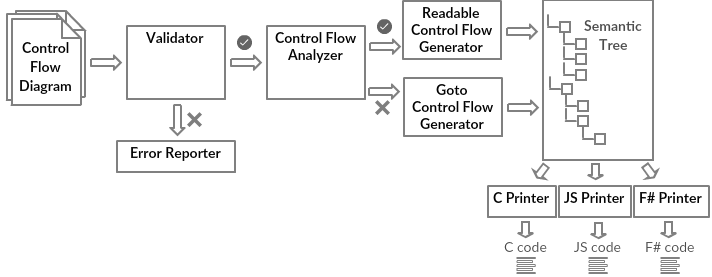
\includegraphics[width=0.6\textwidth]{TS_Generators_Architecture.png}
    \caption{Архитектура подсистемы генерации кода в TRIK Studio}
    \label{image:generatorsArchitecture}
\end{figure*}

На вход генератору поступает визуальная диаграмма. На первом этапе диаграмма обходится в глубину компонентой-валидатором (построенной с применением шаблона проектирования <<посетитель>>). Для всех выражений на встроенном текстовом языке в свойствах блоков происходит их синтаксический разбор и вывод типов. В случае, если диаграмма или код в свойстве содержит ошибки, о них сообщается пользователю в локализованном виде и процесс завершается. В случае, если диаграмма синтаксически корректна, она поступает на вход анализатору потока управления, о котором будет рассказано ниже. В зависимости от того, может ли диаграмма быть сгенерирована в структурированный код, выбирается промежуточный генератор независимого представления, который извлекает семантическое дерева из потока управления диаграммы. Если целевой язык не поддерживает инструкцию \texttt{goto} или, наоборот, высокоуровневые конструкции, как, например, ассемблер-подобный байткод ВМ EV3 (что указывается в конфигурации генератора), соответствующему генератору будет предпочтена его альтернатива. Наконец, на последнем шаге процесса генерации семантическое дерево печатается в целевой текстовый язык. Для этого используется подход с заданием шаблонов генерации для целевого текстового языка. Все, что необходимо сделать для реализации нового генератора --- переопределить набор этих шаблонов и указать конфигурацию генератора. К примеру, шаблон генерации условного оператора в язык C выглядит следующим образом: \begin{verbatim}
    if (@@CONDITION@@) {
        @@THEN_BODY@@
    } else {
        @@ELSE_BODY@@
    }
\end{verbatim}

Вторая из решенных проблем --- модуль анализатора потока управления. В терминах текстовых языков задача звучит так: по данной программе, поток управления которой описан исключительно инструкциями \texttt{goto}, требуется выдать эквивалентную структурированную программу. Данная задача решалась различными исследователями, работающими в области декомпиляции программного кода~\cite{steven1997advanced,деревенец2009структурный}. Приемлемый способ ее решения по методу \textit{интервального анализа} графа потока управления описан, к примеру, в монографии~\cite{steven1997advanced}. Алгоритм интервального анализа графа потока управления диаграммы с незначительными модификациями реализован в TRIK Studio. Коротко опишем его.

Неформально говоря, \textit{интервал} --- это участок графа потока управления с одним входом и одним выходом. Целью алгоритма является построение дерева вложенности интервалов графа потока управления программы, которое в нашем случае и является семантическим деревом. Алгоритм работает на рекурсивном подъеме поиска в глубину в графе потока управления. На каждом шаге алгоритм пробует сопоставить подграф, выходящий из текущей вершины, с каждым из шаблонов элементарных интервалов (алгоритмических конструкций, в терминах которых и будет структурирована программа). Если такой шаблон удается найти, весь подграф сворачивается в одну вершину, и процесс продолжается. Самый простой пример такого шаблона --- два интервала, соединенные ровно одной дугой, что соответствует последовательной композиции. Если на каком-то шаге ни один шаблон не подошел, то диаграмма считается неприводимой.

Очевидным ограничениям на целевой язык в текущей реализации генераторов является его императивность: цепочка блоков на диаграмме должна преобразовываться в последовательное исполнение утверждений в текстовом языке, что проще всего достигается применением оператора последовательной композиции. Тем не менее, идея использования промежуточного шага генерации в независимое представление работает и здесь. К примеру, для поддержки генерации в чисто функциональные языки достаточно расширить элементы независимого представления конструкцией продолжения (continuation passing style, CPS) и добавить промежуточный генератор диаграммы в независимое представление в форме CPS. После этого достаточно переопределить шаблоны печати независимого представления во все необходимые языки.

\section{Textual language parser and interpreter}
\label{chapter:parser}
TRIK Studio uses visual languages for robots programming, but arithmetic expressions, intrinsic function calls and so on are better represented with textual strings (in fact, NXT-G tries to use visual blocks even for arithmetic expressions, representing them as syntax trees, it is very inconvenient). As a textual part of a language for both visual languages TRIK Studio uses a subset of Lua 5.3\footnote{https://www.lua.org/}, customized for our needs. Decision to implement our own parser and interpreter of a textual language was made under these considerations:
\begin{itemize}
	\item we needed a small textual language with lightweight syntax and without explicit typing since it shall be used by non-programmers;
	\item we needed explicit abstract syntax tree and the ability to run type inference on it since we were going to generate code on C or EV3 bytecode, which is strongly typed;
	\item we needed to be able to customize language syntax if the need will arise;
	\item all existing implementations for such languages had interpreter without access to a syntax tree or a parser that was not reusable from C++ code;
	\item since we needed only a subset of a language (arithmetic expressions, without statements, custom function and type definitions), writing custom parser was not a difficult task.
\end{itemize}

Parser and interpreter were implemented as a separate library in QReal core, so the resulting textual language is available not only in TRIK Studio, but in all other domain-specific solutions based on QReal. Parser implementation consists of two parts --- general-purpose parser combinator library and Lua parser library implemented using parser combinators. Many projects use ANTLR\footnote{http://www.antlr.org/}, boost.spirit\footnote{http://boost-spirit.com/home/}, yacc\footnote{http://dinosaur.compilertools.net/yacc/} as tools for parser development, but we once again created our custom solution, mainly to avoid additional external dependencies and complication of a build process --- QReal and TRIK Studio are developed by a large community, and not everyone is happy to install additional tools and learn how to use them, especially if their work has nothing to do with syntax analysis and they are students who do not took formal languages course yet.

QReal parser combinator library supports recursive-descent parsers which are able to parse a subset of LL(1) grammars. FOLLOW($\alpha$) set is not calculated, so it limits the expressiveness of resulting grammars, but we were still able to use Lua 5.3 grammar almost as it is specified, with only minor modifications related to factorization and left recursion elimination, which shall be done anyway for LL parsers. For arithmetic expressions Precedence Climbing\footnote{http://www.engr.mun.ca/\~theo/Misc/exp\_parsing.htm} algorithm was used, and it also required some minor alterations in Lua grammar. Custom modifications were made mainly on lexer level to allow, for example, to use '!=' for inequality in addition to '\verb|~=|' used in Lua. Here is a quick example\footnote{full specification of our parser with many irrelevant technical details see at https://github.com/qreal/qreal/tree/master/qrtext/src/lua} of production written in C++ with our library ("`statement is ';' or a list of expressions, optionally followed by '=' and other list of expressions"'):
\begin{verbatim}
	// stat ::= ‘;’ | explist [‘=’ explist]
	stat = (-LuaTokenTypes::semicolon 
	    | (explist & ~(-LuaTokenTypes::equals & explist)))
\end{verbatim}

\verb|LuaTokenTypes::semicolon| is a token corresponding to ';', operator '-' creates a simple parser that can parse only semicolons and excludes semicolon from AST, "`explist"` is a reference parser object, like "`stat"', defined elsewhere, '\&' combines two parsers into a parser which accepts concatenation of their corresponding strings, '|' combines two parsers into a parser that accepts alternative, '\verb|~|' creates optional parser from its argument, which shall also be a parser. There are also operators for adding semantic actions to productions and assigning parser a name for debug purposes. When all parsers are combined in such a way, it is enough to call 'parse()' method of a resulting parser object, giving it a token stream. Parser combinator library was used for another language in QReal~\cite{tikhonova2015generation}, so it is general enough to support not only Lua.

Parser returns abstract syntax tree on which type inference algorithm is executed, providing types for all variables and expressions. Type inference uses Hindley-Milner-style~\cite{damas1982principal} algorithm, simplified for performance reasons and extended to support overloading and coercion. Type inference is also generalised and Lua type inferer only defines inference rules for Lua-specific AST nodes, core type inference functionality is available for all QReal textual languages.

After type inference is complete, expression is ready to be evaluated by an interpreter. Interpreter allows to register intrinsic functions, also it allows to add custom variables with their values, to support using current sensor values in calculations --- robot communication subsystem receives telemetry data from a robot and injects sensor readings into interpreter, which uses them to calculate expressions.

Last notable feature of parsing/interpreting subsystem is extensive use of caching to avoid parsing or reevaluating expressions as much as possible. Program shall be interpreted in real-time, so reparsing and reevaluating expressions every several milliseconds, as required by many control algorithms, would be severe performance problem. But program can be changed by user during interpretation, values for some variables may be changed by external code, such as sensor readings changed by communication subsystem --- so the interpreter keeps track of changes and uses previously calculated values if possible.

\section{Simulator}
\label{chapter:2dModel}

Особая часть среды TRIK Studio, отделимая от всей остальной системы --- подсистема двумерного имитационного моделирования робота (двумерный симулятор). Окно симулятора встроено в интерфейс TRIK Studio, но может и использоваться отдельно. Основная часть симулятора --- редактор модели мира. В специальном меню можно выбрать инструмент рисования (подобно тому, как это происходит в большинстве графических редакторов). Инструменты рисования делятся на стены (твердые предметы, на которые реагируют ультразвуковые и инфракрасные датчики роботов и сквозь которые робот не может проехать) и цветные маркеры на полу (элементы, на которые реагируют датчики цвета, освещенности и эмуляторы систем видео-зрения) --- прямые линии и кубические кривые безье, прямоугольники, эллипсы и стилус (произвольная растровая фигура, рисующаяся мышью как карандашом). Для каждого маркера на полу может быть задана его толщина, цвет и заливка. Модель робота всегда присутствует на сцене редактора мира, на ней произвольным образом можно размещать виртуальные датчики. Робот представляет собой двухколесную тележку с дифференциальным приводом. Для удобства регионы сканирования датчиков расстояния подсвечиваются. На отдельной панели для каждой поддерживаемой модели робота (NXT, EV3 или TRIK) присутствует эмулятор панели контроллера: фронтальное изображение его лицевой панели с кнопками, нажатие мышью на которые эмулирует нажатие на кнопку реального контроллера, цветными светодиодами, меняющими свой цвет соответственно тому, как того требует написанная пользователем программа, и эмулятором дисплея, изображение на котором можно менять блоками из группы <<Рисование>>.

Важной особенностью симулятора является то, что режим исполнения программы неотличим от режима создания модели мира. Модель мира может редактироваться даже в момент исполнения программы, на любое добавление пользователем стенок и цветных элементов во время исполнения программы датчики начнут реагировать немедленно; положение и направление робота и его датчиков в пространстве может быть изменено в любой момент, что соответствует в реальном мире физическому воздействию на корпус робота.

Симулятор построен на основе архитектуры Model-View-Controller. Модель содержит сериализуемое описание мира и робота, уведомляет о любом изменении любого свойства любого предмета. На события модели подписывается представление, все изменения в модели автоматически отображаются на сцене и панелях симулятора. Пользовательские действия в представлении выполняются через контролирующую компоненту, которая кладет очередное действие на вершину специального стека для возможности его отмены и повтора.

Важной частью модели является ее <<физика>>. В симуляторе реализовано две физические модели поведения робота: идеальная и реалистичная. В идеальной физике игнорируются силы трения о пол и стены, импульсы моторов, при неизменных скоростях моторов робот будет двигаться равномерно (без ускорения и замедления). Любое, даже самое легкое столкновение со стеной в такой модели остановит робота. В реалистичной модели ведется полный учет сил тяги и трения робота о пол и стены, при столкновении со стеной робот поведет себя подобно тому, как это происходит в реальности. Переключение между физическими моделями происходит при выставлении соответствующего флага на панели настроек симуляции и может произойти даже во время исполнения программы. Имеется возможность <<зашумления>> показаний датчиков и импульсов на моторах гауссовым шумом.

Время в двумерном симуляторе не соответствует процессорному: в нем существует централизованная временная прямая, темп хода которой может меняться на специальной панели (что не меняет поведения робота). Та же самая временная прямая используется в интерпретаторах визуальных языков TRIK Studio для соответствия блоков работы со временем модельному, а не процессорному времени.

\section{Automatic checking of solution correctness}
\label{chapter:constraintsChecker}

Последняя важная подсистема, о которой будет рассказано в данной работе --- механизм автоматической проверки заданий на TRIK Studio. Модель мира в двумерном симуляторе может быть превращена специальными средствами среды в упражнение, распространяемое между учениками. Для этого достаточно задать два набора описаний:

\begin{itemize}
    \item описание того, какие части упражнения нельзя менять ученику (модель мира, начальное положение робота и его датчиков, сам набор датчиков, привязку моторов и физические настройки симуляции),
    \item программа проверки корректности решения задачи.
\end{itemize}

Программа проверки ограничений описывается на специальном текстовом XML-подобном языке. Данный язык интересен сам по себе и может рассматриваться как отдельный результат работы. Программа на таком языке представляет собой множество событий $\{ e_1, e_2, ..., e_n \}$, где каждое событие 
$e_i$ представляет собой тройку $(id_i, c_i, T_i)$:

\begin{itemize}
    \item $id_i$ --- идентификатор события: внутренняя метка, по которой другие события могут получать информацию о событии $e_i$, может быть пустым;
    \item $c_i$ --- условие срабатывания события, представляющее собой формулу логики первого порядка без кванторов, об интерпретации предикатных и функциональных символах которой будет рассказано ниже;
    \item $T_i$ --- упорядоченный список элементарных триггеров $[ t_{i_1}, t_{i_2}, ..., t_{i_n} ]$. Элементарный триггер задает действие, выполняемое в момент истинности условия срабатывания события $c_i$.
\end{itemize}

Одно событие задается одним элементом в XML-спецификации программы. Каждое событие в текстовом описании 
программы может быть представлено либо в \textit{каноническом} виде, либо в виде \textit{ограничения}. Событие в канонической форме --- уже описанная тройка $(id_i, c_i, T_i)$.

Событие в форме ограничения --- это тройка $(id_j, c_j, message_j)$. Ограничение интерпретируется как событие $(id_i, $$\neg$$c_i, [ fail(message_j) ])$, где $fail(message_j)$ --- триггер прекращения исполнения имитационной модели с выдачей сообщения об ошибке $message_j$. Другими словами, ограничение --- это событие, которое срабатывает, когда нарушается заданное условие, и которое сообщает пользователю об этом нарушении. Описание события в форме ограничения введено в язык из чисто прагматических соображений, так как на практике удобно описывать утверждения вида <<робот $x$ не должен покидать пределы зоны $z$>> или <<к роботу $x$ должен быть подключен набор датчиков $s$>> именно в терминах ограничений, а не событий. Особый случай такого ограничения --- лимит времени на выполнение программы. Лимит времени должен быть указан в любой программе проверки ограничений имитационной модели TRIK Studio, так как процесс проверки, очевидно, не может осуществляться бесконечное время. Наличие ограничения на лимит времени проверяется как часть синтаксиса языка.

Коротко опишем множество используемых в языке предикатных и функциональных символов и элементарных триггеров. Предикатные символы можно поделить на несколько групп:
\begin{itemize}
    \item Предикаты сравнения значений термов $>$, $<$, $\leq$, $\geq$, $=$, $\neq$.
    \item Пространственные предикаты. Имеют вид <<предмет $x$ находится внутри области $y$>>.
    \item Предикаты состояния событий $settedUp(id_i)$ и $dropped(id_i)$, описывающие состояние события 
            (активно/неактивно). В активном состоянии событие может быть выполнено, в неактивном оно не выполнит триггеры даже при выполнении условия срабатывания события.
    \item Предикат времени $timer(t)$, который становится истинным спустя $t$ отсчетов модельного времени и остается истинным после, а до этого момента ложен.
    \item Прочие предикаты, выражаемые уже описанными и введенные исключительно в целях удобства.
\end{itemize}

Функциональные символы бывают следующих видов:
\begin{itemize}
    \item Константы различных типов (целочисленные, с плавающей точкой, строковые, логические, цветовые, геометрические и пр.).
    \item Символ $variableValue(id)$ для получения значения переменной с идентификатором $id$. Переменные могут быть полезны для реализации сложной логики проверки, например, при подсчете числа проделанных роботом итераций.
    \item Арифметические и геометрические операции над значениями других термов, например, модуль числа, подсчет расстояния между двумя точками или выпуклая оболочка фиксированного множества точек.
    \item Символы сравнения формы двух объектов с использованием расстояния Левенштейна, полезные при проверке схожести фигур, нарисованных роботом и на его дисплее.
    \item Символ $objectState(path)$ --- основное средство получения информации о состоянии устройств робота и свойствах предмета из внешнего мира. Аргумент $path$ --- путь к желаемому свойству в иерархии объектов в модели мира. Такой путь будет преобразован системой в последовательность получений значений свойств объектов C++, реализующих предметы в модели мира посредством механизма рефлексии Qt.
\end{itemize}

Наконец, элементарные триггеры делятся на следующие категории:
\begin{itemize}
    \item $success$, $fail(message)$ --- управление состоянием проверки. Первый помечает результат проверки как успешный, второй --- как неудавшийся, отображая заданное сообщение об ошибке.
    \item Триггеры задания значения переменных и изменения значения свойств элементов имитационной модели мира.
    \item Триггеры управления состоянием событий. Каждое событие может активировать или деактивировать другое событие или себя; с помощью этого можно задавать сложную логику проверки.
\end{itemize}

Пример простейшей программы на языке задания ограничений имитационной модели мира в TRIK Studio приведён в листинге~\ref{code:constraints}.

\captionsetup[figure]{name=Листинг}
\setcounter{figure}{0}

\begin{figure*}[!t]
\begin{verbatim}
<!-- Корневой элемент, означающий начало программы проверки ограничений -->
<constraints>

    <!-- Обязательное в любой программе ограничение на время работы -->
    <timelimit value="2000"/>

    <!-- Ограничение на местоположение робота -->
    <constraint failMessage="Робот покинул допустимую область!">
        <inside objectId="robot1" regionId="myspace"/>
    </constraint>

    <!-- Условие успешности программы: робот должен сказать "Привет" с помощью
        встроенного механизма синтезирования речи и нарисовать улыбку на дисплее -->
    <event settedUpInitially="true">
        <conditions glue="and">
            <equals>
                <objectState object="robot1.shell.lastPhrase"/>
                <string value="Привет"/>
            </equals>
            <equals>
                <objectState object="robot1.display.smiles"/>
                <bool value="true"/>
            </equals>
        </conditions>
        <trigger>
            <success/>
        </trigger>
    </event>

</constraints>
\end{verbatim}
\caption{Пример программы проверки ограничений имитационной модели мира в TRIK Studio.}
\label{code:constraints}
\end{figure*}

Архитектурно система проверки ограничений представляет собой отдельно стоящий модуль, использующий в качестве разделяемых библиотек ядро и имитационную модель системы TRIK Studio. Использование механизма рефлексии Qt для доступа к свойствам объектов имитационной модели позволяет намного проще масштабировать саму модель: при расширении возможностей системы или добавлении новых симулируемых устройств новые объекты и свойства будут немедленно доступны из языка описания ограничений, без дополнительной модификации кода проверяющей системы. Тестовая система подписывается на события имитационной модели подобно тому, как это делает представление симулятора (в смысле архитектуры MVC), и вызывает проверку ограничений на каждом отсчете модельного времени. При этом проверяются только активные ограничения, которых на практике в каждый конкретный момент времени немного, поэтому общая скорость работы симулятора при наличии проверяющей программы практически не меняется.

Описанный язык удобен для задания пространственных и временных ограничений на поведение системы. Он является значительно более удобным и выразительным, чем, к примеру, язык темпоральных логик или топологико-темпоральных логик, используемых для описания формальных ограничений на поведение робота в работах последних лет~\cite{mordvinov2016formal,kress2007s,бугайченко2007разработка,дмитриев2013адаптация}. При этом язык не тьюринг-полон (на нем, к примеру, нельзя выразить нормальные алгоритмы Маркова из-за отсутствия в языке средств работы с коллекциями произвольной длины, что делает невозможным реализацию на нем замены в строке), это говорит о возможности автоматического анализа интересных свойств программ на нем. Ко всему прочему, подмножество этого языка может использоваться для описания требований к программе для последующей ее формальной верификации. В будущих версиях TRIK Studio планируется реализация визуального конструктора ограничений на этом языке. Появление такого конструктора и интеграция мощного верификатора дадут возможность формально доказывать корректность визуальных программ, не написав ни одной формулы формальной логики. Подробное исследование этого вопроса --- тема для будущих работ.

Система проверки ограничений используется для функционального тестирования среды на сервере системы непрерывной интеграции. Об автоматизированном тестировании среды TRIK Studio подробнее рассказано в работе~\cite{mordvinov2016testing}.

This functionality is also used as an automatic checker of exercises for MOOC on Stepik platform\footnote{https://stepik.org/s/7qe3xj4Z}. Without such checker it would be impossible to provide feedback to possibly large number of students, making course much less interactive. From a technical point of view checker is a set of scripts which launch "`headless"' interpreter (i.e. interpreter without GUI) on a correct field with correct constraints. Checker is hooked up into Stepik infrastructure and runs in a separate Docker\footnote{https://www.docker.com/} container when new solution is submitted. Checker has several fields and corresponding constraint descriptions for each task (from one to five), each solution is checked against all those fields to test that it works in different situations and is not hardcoded. Fields are hidden from the user but error reporter output does gets displayed, so students can guess what went wrong (well, theoretically. But it's better than traditional ACM ICPC system, where only a number of incorrect test and a general type of error are reported).

Checker can also send a visual representation of a field with a trace of a robot to a client. Trace consists of points of a robot trajectory and values reported by its sensors, and this trace can be played back by a web application described in~\cite{zakharov2016web} (in Russian). This web application also allows to actually create solutions for almost all tasks from the course right in the browser, form a correct TRIK Studio save file and run it on a server on checker, playing back the result, so a student perceives this as "`TRIK Studio in a browser"'. This application works standalone, but is not integrated into Stepik course yet due to technical difficulties related to Stepik infrastructure.

\section*{Conclusion}
\label{chapter:conclusion}

В статье было дано техническое описание среды программирования роботов TRIK Studio. Среда разработана на кафедре системного программирования Санкт-Петербургского Государственного Университета и по данным системы Google Analytics в настоящее время насчитывает около десятка тысяч пользователей на всех обитаемых континентах мира. На данный момент интерфейс среды переведен на три языка (русский, английский, французский), в том числе силами сообщества пользователей. Система активно развивается, исходный код среды находится в открытом доступе\footnote{https://github.com/qreal/qreal (дата обращения: 14.05.2016)}. Без учета ядра DSM-платформы, код системы содержит порядка 100 тысяч строк, включая техническую документацию всех компонентов, написанную в doxygen\footnote{http://www.doxygen.org/ (дата обращения: 14.05.2016)}-формате в заголовочных файлах кода среды.

Будущие направления работы разделяются на два больших класса: технические улучшения среды и исследовательские проекты. Задачи из первого класса появляются из общения с педагогами и учениками, пользующимися средой, этих задач довольно большое число (на системе управления процессом разработки их записано порядка сотен). К примеру, это задачи по поддержке новых робототехнических платформ в среде (таких, как, Arduino), улучшение двумерного симулятора (доработка физической модели, поддержка симуляции мультиагентных систем и т.д.), поддержка новых текстовых языков, общие улучшения ядра DSM-платформы QReal и т.д. Задачи из второго класса рассматривают TRIK Studio как исследовательскую платформу и требуют применения теоретических научных работ в области компьютерных наук. На данный момент исследовательская работа идет по двум <<ветвям>>: ветви предметно-ориентированного визуального моделирования и ветви формальных методов анализа программных систем. К первой ветви относится, к примеру, работа по автоматической генерации метамодели потокового языка из описания доступных пакетов системы промежуточного уровня на роботе (такой, как ROS~\cite{quigley2009ros}). В рамках второго направления ведутся работы по выражению строгой семантики языков с целью применения подходов к формальной верификации диаграмм.

\bibliographystyle{utf8gost705u}
\bibliography{trikStudioEnglish}

\end{document}